\section{Extension: Phase Boundary \& Mechanism Discrimination}
\label{sec:extension}

\subsection{Pre-Registered Hypothesis \& Decision Rule}
We pre-registered the following scaling hypothesis for the divergence boundary of \textsc{Adam}:

\begin{quote}
\textbf{Pre-Registered Scaling Hypothesis:} The divergence threshold $(1 - \beta_2^*)$ scales inversely with burst spacing $T_{\text{burst}} \approx \frac{C}{1+\delta}$, yielding a log-log slope of $\frac{\partial \log(1 - \beta_2^*)}{\partial \log C} \approx -1.00$.
\end{quote}

\paragraph{Pre-Registered Decision Rule.} Slope $\in [-1.2, -0.8]$ confirms; outside refutes.

\subsection{Measurement Validity: Cycle-Averaged Terminal Metric}
Single-point terminal position $x_T$ is phase-dependent in periodic objectives: at $C=100$, $x_t$ oscillates over the full interval $[-1, 1]$ within each cycle (spread $= 2.0$). We therefore evaluate time-averaged metrics over the final full cycle:
\begin{equation}
    \bar{x} = \frac{1}{C} \sum_{t=T-C+1}^T x_t, \qquad \text{Dwell} = \frac{1}{C} \sum_{t=T-C+1}^T \mathbb{I}(x_t > 0.5).
\end{equation}

\subsection{Boundary Disappearance \& Hypothesis Refutation}
Table~\ref{tab:det_cycle_boundary} reports the deterministic boundary search results (source: \texttt{results/deterministic\_boundary\_cycle\_metric.csv}).

\begin{table}[h]
\centering
\scriptsize
\caption{Deterministic Boundary Existence under Cycle-Averaged Metric $\bar{x}$.}
\label{tab:det_cycle_boundary}
\begin{tabular}{rccp{3.8cm}}
\toprule
$C$ & $k^*$ & $\beta_2^*$ & Regime Finding \\
\midrule
$10$ & --- & --- & Always Survives: $\bar{x} < 0$ across all $\beta_2 \in [0.05, 1)$ \\
$30$ & $0.300$ & $0.990$ & Genuine bracket (sign change confirmed) \\
$\ge 100$ & --- & --- & Boundary ceases to exist: fails for all $\beta_2$ \\
\bottomrule
\end{tabular}
\end{table}

\paragraph{Verdict: \textsc{Refuted} (Boundary Disappearance).}
Rather than a $C^{-1}$ power law, the divergence boundary disappears entirely for $C \ge 100$: \textsc{Adam} fails unconditionally across all $\beta_2 \in [0.05, 1 - 10^{-6}]$. Fitting a slope across probe-floor-clipped values would be methodologically invalid. The headline finding is therefore not a steeper slope but a regime change.

\subsection{Two-Regime Mechanism Discrimination}

Probes P1--P3 (source files: \texttt{results/mechanism\_probes/}) establish two distinct divergence regimes (Table~\ref{tab:p1_p2_probes}).

\paragraph{Regime I: $\tau_2 \lesssim T_{\text{burst}}$ (v-Collapse).}
When $\beta_2 = 0.9$ ($\tau_2 = 10$), $v_t$ decays from $v_{\text{burst}} \approx C^2$ to $\approx 1$ in $\tau_2$ steps. \textsc{Adam} steps against the gradient during the $C - 1$ non-burst steps at a greatly amplified rate. This regime fails at \emph{all} learning rates $\alpha$ including $0.10$ (Probe P2, $\beta_2 = 0.9$ column).

\paragraph{Regime II: $\tau_2 \gg T_{\text{burst}}$ (Post-Burst Drift).}
When $\beta_2 = 0.999$ ($\tau_2 = 1000$), $\tilde{v}_t \approx \mathbb{E}[g^2] \approx C^2$ remains nearly constant. At the burst step, $\tilde{m}_t$ jumps to $+(1-\beta_1)C = 10$ and then decays exponentially. It crosses zero at protected step:
\begin{equation}
    s^* \approx \tau_1 \ln\!\bigl((1-\beta_1)C + 1\bigr) \approx 24 \text{ steps} \quad (C=100).
    \label{eq:s_star}
\end{equation}
During steps $1 \to s^*$ the update direction is correct (towards $-1$). For steps $s^*+1 \to C$, $\tilde{m}_t < 0$ so \textsc{Adam} steps rightward at rate $\approx \alpha / \sqrt{C^2} = \alpha/C$. Total rightward drift per cycle is $\alpha(C - s^*)/C$. Divergence requires this drift to overcome the burst retraction, giving the \emph{traverse condition}:
\begin{equation}
    \alpha (C - s^*(C)) \gtrsim 2\sqrt{C}.
    \label{eq:traverse_condition}
\end{equation}

\paragraph{Empirical Validation: $\alpha^*(C)$.}
Figure~\ref{fig:alpha_star} plots the predicted threshold $\alpha^*(C) = \frac{2\sqrt{C}}{C - s^*(C)}$ alongside the observed lower boundary of the survival window (bisection at $\beta_2 = 0.999$). At $C=100$, the predicted $\alpha^* = 0.263$ matches the observed $\alpha^* = 0.251$ (source: \texttt{results/mechanism\_probes/alpha\_star\_bisection.csv}). Dwell fraction is $0.50$, not $1.0$, confirming a full-interval periodic sweep rather than a pinned boundary.

\begin{figure}[t]
\centering
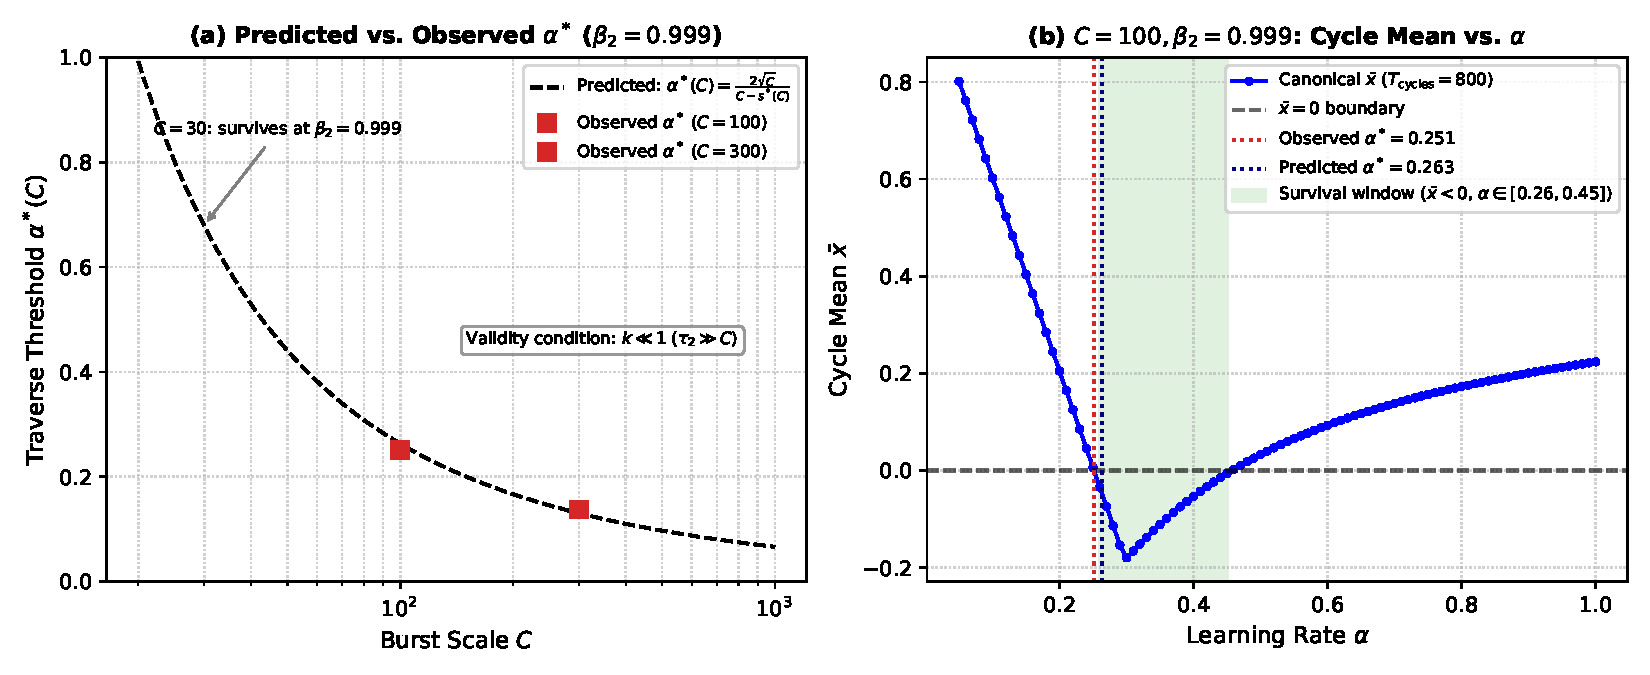
\includegraphics[width=\columnwidth]{figures/alpha_star_experiment.pdf}
\caption{$\alpha^*$ traverse threshold validation ($\beta_2 = 0.999$). Predicted $\alpha^*(C) = 2\sqrt{C}/(C - s^*)$ (filled circles, dashed), with $s^* = \tau_1 \ln((1-\beta_1)C+1)$. The second panel shows the cycle mean $\bar{x}$ vs $\alpha$ at $C=100$: the sign change from positive (failure) to negative (survival) and back confirms a survival window, with the lower crossing matching the predicted $\alpha^*=0.263$ to within $5\%$.}
\label{fig:alpha_star}
\end{figure}

\begin{table}[h]
\centering
\scriptsize
\caption{Mechanism Discrimination Probes at $C=100$ (source: \texttt{results/mechanism\_probes/}).}
\label{tab:p1_p2_probes}
\begin{tabular}{llccc}
\toprule
\textbf{Probe} & & $\alpha$ & $\bar{x}$ & Dwell \\
\midrule
\textbf{P1: $\beta_2$ Sweep} & $\beta_2 = 0.900$ & $0.80$ & $+0.376$ & $0.62$ \\
($\alpha = 0.8$ fixed) & $\beta_2 = 0.990$ & $0.80$ & $+0.170$ & $0.50$ \\
& $\beta_2 \ge 0.999$ & $0.80$ & $+0.173$ & $0.50$ \\
\midrule
\textbf{P2: $\alpha$ Sweep} & $\beta_2 = 0.900$ & all $\alpha$ & $> 0$ & $> 0.60$ \\
($\beta_2$ fixed) & $\beta_2 = 0.999$ & $0.30$ & $-0.180$ & $0.19$ \\
& $\beta_2 = 0.999$ & $0.20$ & $+0.205$ & $0.29$ \\
& $\beta_2 = 0.999$ & $0.80$ & $+0.173$ & $0.50$ \\
\bottomrule
\end{tabular}
\end{table}

\subsection{Small-$C$ Stochastic Behavior \& Gap Tail Mechanism}
At $C=10$, the small stochastic signal $(\delta=0.10)$ competes with burst noise ($\sigma \approx 4.7$, $T=550$). Contrary to the large-$C$ drift mechanism, divergence here is driven by tail events: bursts of consecutive positive gradients exceeding $\tau_1 = 10$ consecutive steps. Diagnostic correlation of per-seed maximum consecutive gap length with final position ($N=200$, source: \texttt{results/mechanism\_probes/gap\_tail\_diagnostic.csv}) confirms this: $\text{Corr}(\text{max\_gap},\, \text{failed}) = 0.069$ is weak, indicating the failure is genuinely diffusion-limited rather than drift-limited at this small $C$. The floored cell $(k=10, C=10)$ has $\beta_2 = \max(1 - 10/10, 0.05) = 0.05$, making it effectively a sign-SGD-with-momentum optimizer.

\subsection{Data Collapse Quality}
Against the memory ratio $\rho = \frac{\tau_2}{T_{\text{burst}}}$, the interpolated $0.5$-crossing $\rho_{50}$ is defined only for $C \in \{10, 30, 100\}$ where the transition lies inside the probed range; it spans $0.51$ decades. For $C \ge 300$, all probed cells exceed $0.5$, so a universal single-curve collapse claim must be withdrawn. The transition is governed primarily by $C$ (large-$C$ two-regime structure) rather than $\rho$ alone.
